\documentclass[11pt]{article}
\usepackage{amsmath, amssymb, amscd, amsthm, amsfonts}
\usepackage{graphicx}
\usepackage{hyperref}
\usepackage{commath}
\usepackage{subfig}
\usepackage{float}
\usepackage{natbib}
\oddsidemargin 0pt
\evensidemargin 0pt
\marginparwidth 40pt
\marginparsep 10pt
\topmargin -20pt
\headsep 10pt
\textheight 8.7in
\textwidth 6.65in
\linespread{1.5}

\title{Economics Influence on Housing price Index within Southeast Asian Countries}
\author{Steven Qin\\20819760\\s45qin@uwaterloo.ca \and Tiankai Jiang\\20834939\\t57jiang@uwaterloo.ca}

\date{\today}

\newtheorem{theorem}{Theorem}
\newtheorem{lemma}[theorem]{Lemma}
\newtheorem{conjecture}[theorem]{Conjecture}

\newcommand{\rr}{\mathbb{R}}

\newcommand{\al}{\alpha}
\DeclareMathOperator{\conv}{conv}
\DeclareMathOperator{\aff}{aff}

\makeatletter
\setlength{\@fptop}{0pt}
\makeatother

\begin{document}

\maketitle

\section{Introduction \& objective}\label{section-introduction}
For the purpose of this project, the objective is to consider various macroeconomic factors, such as the interest rate, GDP growth rate, Consumer Confidence Index (CPI), with an effect on the country wide housing price index. We would subjectively select four individual Southeast Asian countries suitable to represent the overall four national economics level categories ranked by the World Bank. Giving the covid-19 contingency around the world, we would also like to make certain adjustment to the model used to seek a hint on the overall cross-sectional impact.

Target Countries: Japan, People’s Republic of China, Philippine, and Nepal (In descending order of the economics level).

\section{Proposed Model}\label{section-proposedmodel}
$y = \beta_0 + \beta_1x_1 + \beta_2x_2 + ... + \beta_nx_n + \epsilon$

Initially, we choose total population, population density, urban population percentage, unemployment rate, real estate activities, taxes on property, per capita GDP, household final consumption, interest rate\citep{10.2307/23606731, 10.2139/ssrn.2431627, aei297454} as independent variables($x_i$). Dependent variable($y$) is the house price index.

\section{Modeling data}\label{section-proposedmodel}
In this section, we plan to briefly walk through the data modeling and analysis steps which will contribute towards the final delieverable. Using the data from USA as an example, we collected the data of the annual housing price index, GPD per capital, Unemployement rate, and number of building permits.

\begin{figure}[H]
\captionsetup[subfigure]{labelformat=empty}
\centering
\subfloat[]{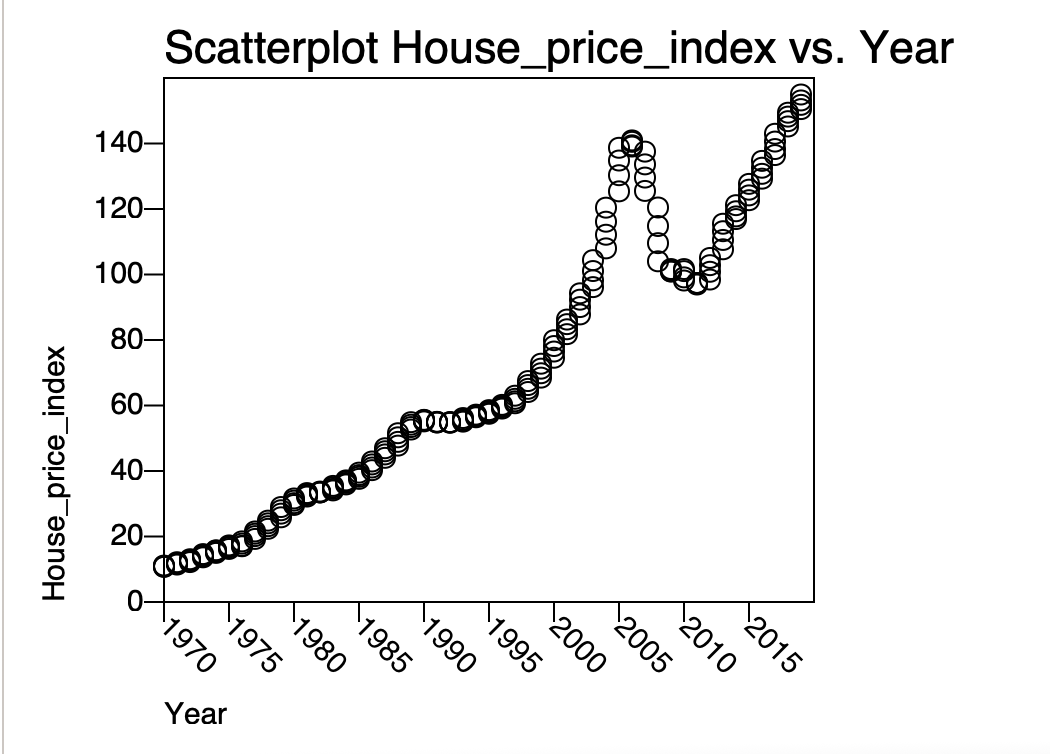
\includegraphics[width=0.24\textwidth]{./image/price_index.png}}
\subfloat[] {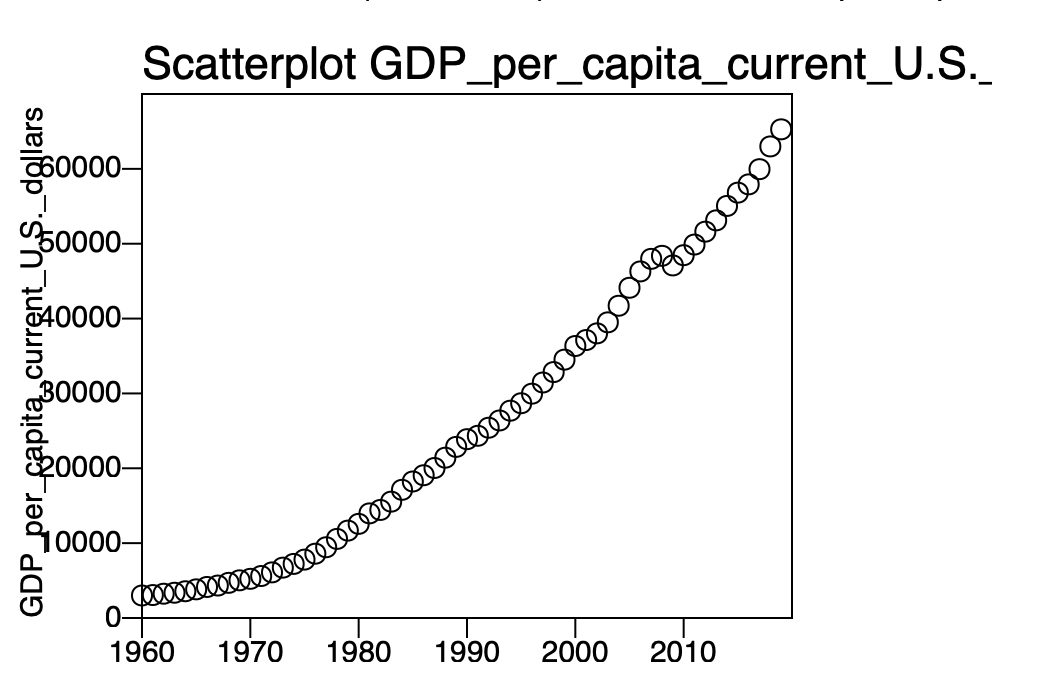
\includegraphics[width=0.24\textwidth]{./image/Gdp.png}}
\subfloat[] {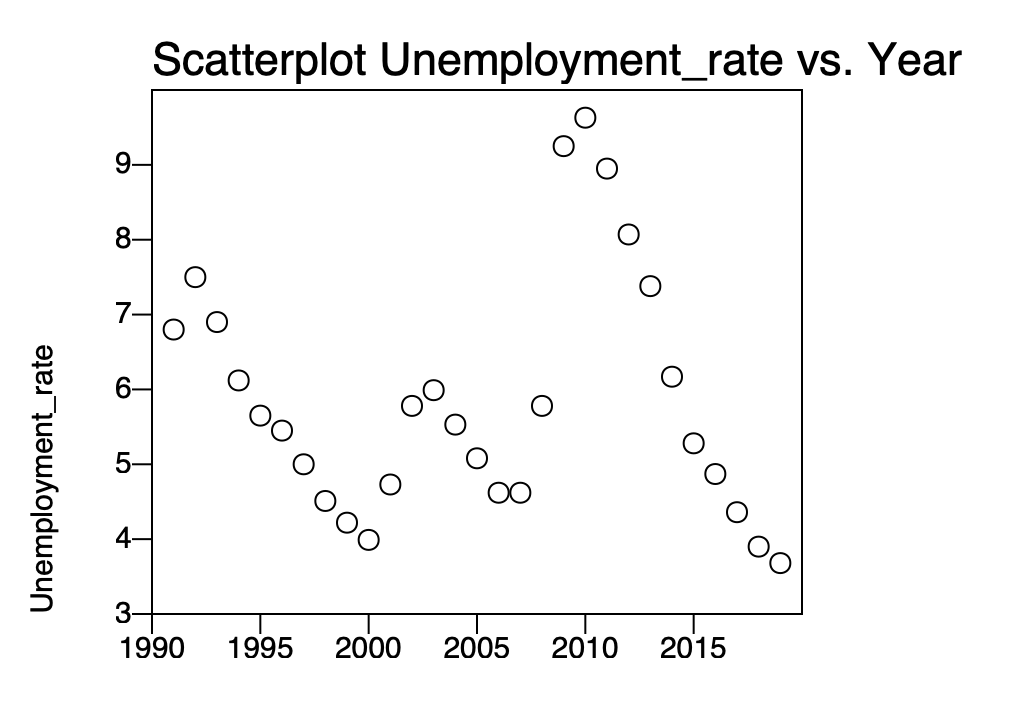
\includegraphics[width=0.24\textwidth]{./image/Unemployment.png}}
\subfloat[] {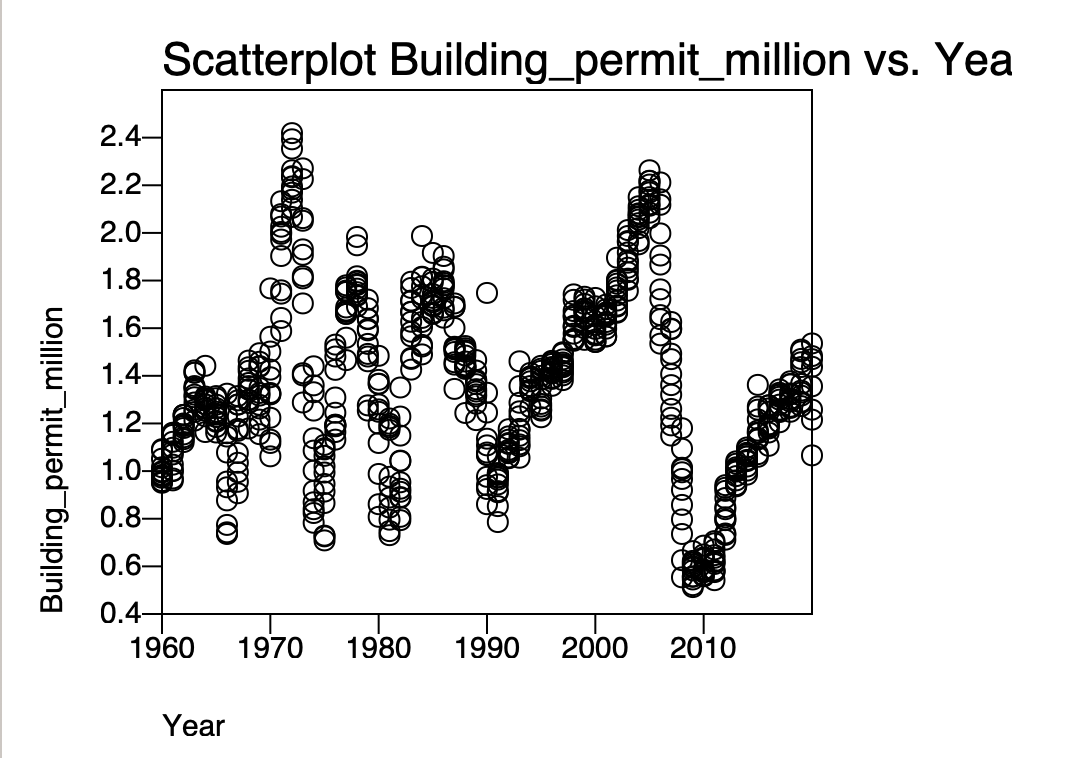
\includegraphics[width=0.24\textwidth]{./image/building_permit.png}}
\end{figure}

As shown above, the housing price has an overall uptrend, with a periodic recession during the 2008 financial crisis. A similar pattern appeals to the growth of GDP per capita. On the other hand, the national unemployment rate and the number of issued building permits are cyclical under the influence of the national economic, world economic environment, and other factors. Although displayed differently, we can still capture similarity characteristics. For instance, unemployment is recorded at a historical high during the financial crisis(The unemployment rate is a lagging indicator of the business cycle. Therefore, we see the historical high is recorded in 2010, but the upward trend obviously ggstarted at approximately coincide with the crisis). In the same way, a pattern can also seem for building permits. 
Hence, we will choose these three mentioned factors as the independent variables for the HPI in the model and analysis of the data based upon it.  

\section{Data Tables and variable discription}\label{section-datatable}
\section{Certainty of Variable}\label{section-Certainty}
HPI is a commonly used indicator by investors to keep a palus on the broader economic trend. The rise and fall is interrelated with the economic. In general, price rise may be interpreted as a form of accumulating wealth from the day-to-day operation. Hence such events often leads to lower unemployment rate and high Consumer Confidence Index (CCI) that leads to high consumptions. Furthermore, it paves the way for a boost in the domestic aggregate demand and GDP. In purpose of this project, my team would select independent variables that have direct implications on the domestic household disposable income level. Factors choosen are listed and described below. 
\begin{itemize}
\item Demand variables: GDP in the form of \(GDP = C + I + G - (X-M)\) where is C is household consumption, I is private domestic investment, G is net government expenditure, X-M represents the net of export. 
\item Price variables: CPI and GDP deflator where as \(deflator = (Nominal GDP / Real GPD) * 100 \)
\item Interest rates: \(real interest rate = nominal interest rate - inflation rate\) where the inflation rate captures the percentage change in the CPI and nominal interest rate shows the domestica policy rate set by each domestic monetary agency. 
\item Mortgage loan and unemployment rate as representation of CCI
\end{itemize}     


\bibliographystyle{apalike}
\bibliography{references}
\end{document}